
\documentclass[conference]{IEEEtran}
\usepackage{stmaryrd}
\usepackage{amsfonts}
\usepackage[boxed, vlined]{algorithm2e}
\usepackage{listings}


% If the IEEEtran.cls has not been installed into the LaTeX system files,
% manually specify the path to it: e.g.,
% \documentclass[conference]{../sty/IEEEtran}

\usepackage{graphicx,times,amsmath} % Add all your packages here

% correct bad hyphenation here
\hyphenation{op-tical net-works semi-conduc-tor IEEEtran}

\IEEEoverridecommandlockouts    % to create the author's affliation portion
                % using \thanks

\textwidth 178mm    % <------ These are the adjustments we made 10/18/2005
\textheight 239mm   % You may or may not need to adjust these numbes again
\oddsidemargin -7mm
\evensidemargin -7mm
\topmargin -6mm
\columnsep 5mm

\begin{document}


% paper title: Must keep \ \\ \LARGE\bf in it to leave enough margin.
\title{\ \\ \LARGE\bf Group 4: System Call Monitor\thanks{Joseph Roth and Scott Klum are with the Department of Computer Science and Engineering at Michigan State University (email: \{rothjos1, klums\}@cse.msu.edu).}}

\author{Joseph Roth and Scott Klum}

% avoiding spaces at the end of the author lines is not a problem with
% conference papers because we don't use \thanks or \IEEEmembership
% use only for invited papers
%\specialpapernotice{(Invited Paper)}

% make the title area
\maketitle

\begin{abstract}
In this paper, we design, implement, and evaluate a basic instrumentation of kernel system calls.
We add the functionality to store information about generic system calls and then hook up a few interesting calls to observe.
A loadable kernel module is used to add to the \textit{proc} file system a means of viewing the statistics about system call usage.
The work is easily extensible to any system call.
\end{abstract}

% no key words

\section{Introduction}

\PARstart{S}{ystem calls} are used by user programs to request protected services from the operating system through the kernel.
The services can range from hardware interaction to process creation to communication setup.
Due to security reasons, these services require the use of privileged instructions which can only be used by the kernel itself.
As such, the kernel provides access to these services through simple system calls.
On the $2.6.32.5$ version of linux used for the project, there are $336$ different system calls.

Our work began as the desire to implement a simple chat service between users on the computer.
We quickly identified that most linux distributions ship with this implemented by either the \textit{talk} or \textit{wall} commands.
Our idea then shifted to creating an extension for this service by saving the most recent chat messages for future retrieval.
In order to save the chat messages in the kernel, we need to identify what system calls the \textit{wall} application uses and capture the message as it gets sent through the kernel.
This idea of identifying an application as it makes system calls then transformed into the main focus of our work as we look at instrumenting the kernel.

In our project proposal, we set out to store data regarding which user and image frequently make use of various system calls in the kernel.
The idea was to start with the calls used by \textit{wall} and place hooks in each of these to capture statistics.
Time permitting, we would continue to poke around the kernel and locate other calls to instrument related to network or disk access.

The motivation for the work is twofold.
First, by monitoring the system call usage, we can identify bottlenecks or resource consuming images which could be removed from the system.
Some of these images may in fact have security vulnerabilities or be malicious in nature.
Second, the motivation is to provide good familiarity with the kernel by giving the developers of this project a wide access to different parts of the kernel.

In section~\ref{sec:background}, we talk about the related work and provide resources used to help with programming.
Then in section~\ref{sec:design}, we give an overview and detailed design of the various components.
We follow this in section~\ref{sec:evaluation} with an evaluation of the software and sample output.
Finally, we briefly draw some conclusions in section~\ref{sec:conclusions}.

\begin{figure}[*]
\begin{lstlisting}
void addNewRecord(char *comm, int uid, char *sys_call, int sys_call_index)
{
        recordPointer[sys_call_index]++;
        strcpy(record[sys_call_index][recordPointer[sys_call_index]].comm,comm);
        strcpy(record[sys_call_index][recordPointer[sys_call_index]].sys_call,sys_call);
        record[sys_call_index][recordPointer[sys_call_index]].uid = uid;
        if (recordPointer[sys_call_index] >= MAX_RECORDS) recordPointer[sys_call_index] = 0;
        if (sysCallPointer >= 0) {
                for (i = 0; i < MAX_SYS_CALLS; i++) {
                        if (strcmp(record[i][0].sys_call,sys_call) == 0) { // Only do if initialized, and the sys_call is equal
                                sysCallPresent = true;
                                if (recordPointer[i] >= 0) {
                                        for (j = 0; j < MAX_RECORDS; j++) {
                                                if ((strcmp(record[i][j].comm,comm) == 0) && (record[i][j].uid == uid)) {
                                                        recordPresent = true;
                                                        record[i][j].count++;
                                                        break;
                                                }
                                        }
                                }
                                if (!recordPresent) {
                                        addNewRecord(comm,uid,sys_call,i);
                                        break;
                                }
                        }
                }
                if (!sysCallPresent) addNewSysCall(comm,uid,sys_call);
        }
}
\end{lstlisting}
\end{figure}

\section{Background}
\label{sec:background}
Instrumentation is not a new subject.
Instrumentation is the process of injecting small amounts of code into an application or system that monitors and records the performance and usage of different parts of code.
This analysis can identify bottlenecks where optimizations can produce dramatic speedup, or security holes where unexpected code is being executed.
Moore \textit{et. al.} compare direct kernel instrumentation with passive network monitoring with the conclusion that better statistics can be derived from direct kernel instrumentation~\cite{cit:1}.

To implement the \textit{proc} file and loadable kernel module, we use a tutorial provided by ``The Geek Stuff'' blog~\cite{cit:2}.
They provided sample code for a simple file where you can write to the file and then later read the text through reading the file.
We only need to use the reading operation, but we also used the sample makefile to create the loadable kernel module as well as the command line instructions to install or remove the module.
Our project also required us to buffer the output into multiple calls since it was too large for a single buffer.
We used the seq\_file interface and used the documentation provided through the linux kernel module programming guide~\cite{cit:3}.

\begin{algorithm*}[t!]
\begin{verbatim}
System call:           write
Image:            bash UID: 0000 Count:           51
Image:   rs:main Q:Reg UID: 0000 Count:           23
Image:            sshd UID: 0000 Count:           91
Image:           dmesg UID: 0000 Count:           749
Image:    avahi-daemon UID: 0104 Count: ++++++++++17109

System call:            read
Image:            bash UID: 0000 Count:           53
Image:        rsyslogd UID: 0000 Count:           1
Image:            sshd UID: 0000 Count:           96
Image:           dmesg UID: 0000 Count:           1
Image:    avahi-daemon UID: 0104 Count: ++++++++++5264
Image:              ls UID: 0000 Count:           8
Image:             cat UID: 0000 Count:           4
Image:         portmap UID: 0001 Count:           7

System call:           close
Image:            bash UID: 0000 Count: ++++++++++65
Image:           dmesg UID: 0000 Count: +         7
Image:              ls UID: 0000 Count: ++        13
Image:             cat UID: 0000 Count: +         10
Image:         portmap UID: 0001 Count:           3

System call:            open
Image:           dmesg UID: 0000 Count: +++++     5
Image:              ls UID: 0000 Count: ++++++++++10
Image:            bash UID: 0000 Count: ++++      4
Image:             cat UID: 0000 Count: +++++++   7
Image:         portmap UID: 0001 Count: +++       3
\end{verbatim}
\caption{Sample output from \textit{proc} file}
\end{algorithm*}

\section{Design and Software Development}
\label{sec:design}
We now present the basic design of our software as well as the implementation details.
To effectively implement an instrumentation, we need a data structure for storing the statistics, a simple code modification to record each system call, and a useful display of the statistics recorded.
Figure~\ref{fig:figure} demonstrates the basic flow of storing to the custom data structure and displaying the results to the user.

\begin{figure}[t!]
  \begin{center}
    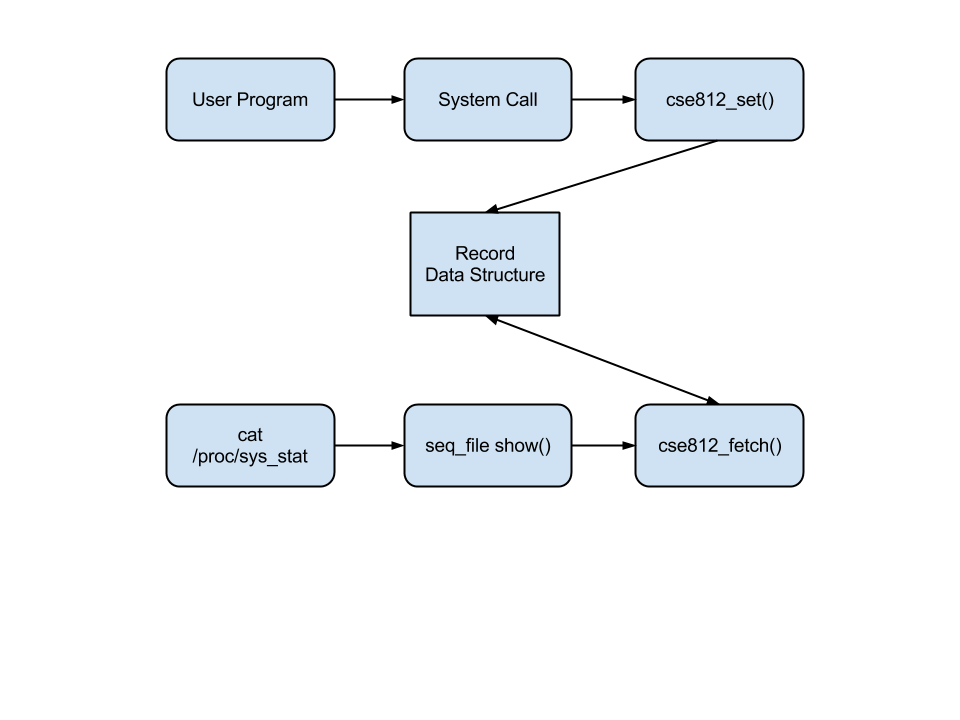
\includegraphics[trim=120 230 90 50, clip, width=1.0\linewidth]{figure.png}
    \vspace{-0.18in}
  \end{center}
  \caption{Flowchart of program flow.}
  \label{fig:figure}
\end{figure}

\subsection{Loadable Kernel Module}
We leverage an LKM to easily insert a proc file to our system, and provide it with a custom read operation.
Each time the LKM is loaded or unloaded, the \textit{cse812\_clear()} function is called to initialize or reset statistics.
We use this function to prevent system calls from being recorded constantly.
That is, without calling the \textit{cse812\_clear()} function when inserting the module statistics are not recorded.

\subsection{Data Structure}
To record the system call, we add a new file, \textit{kernel/sys\_stat.c}, to the kernel which contains two external functions.
One function, \textit{cse812\_clear()}, starts or resets the statistics.
The other function, \textit{cse812\_set(char *, int, char *)}, accepts a tag, user id, and system call name respectively.
The tag is always the calling process image name.
To store the recorded calls, we created our own custom data structure which houses the counts of each call based on the tag, user id, and system call name.
The data structure is essentially a 2-dimensional array of structs which record the needed information.
The first dimension is of size $16$ and is unique for each system call used.
The second dimension is of size $1024$ and is used to store the count for a unique combination of user id and tag.

When the \textit{cse812\_set()} function is called, the data structure is searched first for a match in terms of the system call.
If a match is not found, then a new array of records is created, if all $16$ records have already been used, then it uses a \textit{FIFO} replacement scheme.
In practice, one should ensure that enough records are present to handle all desired system calls.
Once a match is found, then the second dimension is searched for the a match on both the tag and the user id.
The same procedure is used if none are currently found with \textit{FIFO} replacement as well.
Once a final match is identified, the count of calls is incremented by one.

\subsection{Code Injection}
All system calls go through a common entry point in assembly.
Our initial vain though was to hook into this common entry point and be able to record for all system calls at the source.
Since our knowledge of C was rusty, attempting to edit the assembly would be a silly idea.
We still wanted to satisfy one of the most important considerations of instrumentation which is to have minimal impact on the natural code.
We designed a single line of code which can be inserted into the code for any desired system call which will perform the recording.

\begin{verbatim}
cse812_set(current->comm, current_uid(),
    "call name");
\end{verbatim}

\subsection{Display}
Recording the statistics may be the difficult step, but the important step is being able to view the statistics that have been collected.
We implemented the output through the standard means of the \textit{proc} file structure.
We add the \textit{proc} file through the means of a loadable kernel module.
When the module is loaded, the statistic recording is activated and the proc file is created.
To view the statistics, one simply needs to write out the contents of the file through:

\begin{verbatim}
cat /proc/sys_stat
\end{verbatim}

\subsection{Errors}
During the development of our instrumentation method, we encountered two bugs that are instructive.

As one might expect, performing a bad access of a portion of the record array causes the kernel to crash (e.g. indexing into the array beyond its size).
Surprisingly, there were situations in which this caused the kernel to hang rather than crashing and rebooting.
We speculate that this is because the memory being access was such that, while the kernel was aware something was going wrong, the kernel had been trapped in an infinite loop by the bad access.

A more interesting and informative bug occurred after adding a hook for the write system call.
During development, multiple \textit{printk} statements existed in the portion of the code that recorded system calls.
Although we knew that the messages sent to the \textit{printk} function could be accessed via the \textit{dmesg} command, we were unaware that \textit{printk} also logged its data to \textit{/var/log} via the syslog daemon.
This behavior caused the write system call to be executed repeatedly, resulting in a kernel hang (via an infinite loop).

All code written for this project is included in the attached zip file

\section{Evaluation}
\label{sec:evaluation}
In this section, we demonstrate the results of our project in terms of the output from the \textit{proc} file, the efficiency impact on the machine, and interesting notes on the usage of system calls.

A sample output is displayed in the poorly named algorithm 1.
The output is arranged by system call.  Currently, we are monitoring the read, write, open, and close calls.
We display the image name, user id, visual count, and numerical count for each unique pair of images and user ids.
The visual count is a pseudo-histogram of the relative frequencies for each call.
It lets the user immediately identify the most frequent callers.

We make the following observations about the results presented in the sample display.
There are more \textit{close} operations that \textit{open} calls.
We hypothesize that since forked processes retain the open file table, that each child process will have to close a file that was never opened by that process.
The process \textit{avahi-daemon} appears to be making a significant number of reads and writes.
A quick google search demonstrates that this daemon scans the network to identify printers, hosts, or other devices.
To improve system performance, we could either reduce the frequency of this scan, or entirely disable it from scanning.

\textbf{Efficiency:} We make no direct comparison of system performance before and after the additions, but we do make the following claim to performance.
During normal usage, we notice no impact on the speed or responsiveness, but when performing intensive operations, such as compiling the kernel, we do notice a significant impact on the overall speed of compilation.
The use of hash tables instead of searching through an array would alleviate the burden of our instrumentation by allowing for $O(1)$ recording time instead of $O(n*m)$ recording time, where $n$ refers to the maximum number of system calls and $m$ refers to the maximum number of unique combinations.

\section{Conclusions}
\label{sec:conclusions}
In this work, we have demonstrated a means of monitoring specific system calls through the injection of a single line of code into the beginning of each desired system call.
We designed and implemented a simple function to record system calls through the use of a custom data structure.
We created a loadable kernel module to display the statistics through the \textit{proc} file system.

Throughout the process, we learned a lot about the kernel in general.
Neither of us had any experience with kernel development in the past.
This project allowed to to experience a variety of different tasks as well as look at a large portion of code to identify the correct and best spots to place our instrumentation hooks and code.
We both learned tremendous amounts about the kernel and were glad to partake of this project.

Like all good operating systems papers, we now present the real implementation of our project.
We simply changed a single bit in the task struct which caused the rest of the details to fall into place.

% trigger a \newpage just before the given reference
% number - used to balance the columns on the last page
% adjust value as needed - may need to be readjusted if
% the document is modified later
%\IEEEtriggeratref{8}
% The "triggered" command can be changed if desired:
%\IEEEtriggercmd{\enlargethispage{-5in}}

% references section
% NOTE: BibTeX documentation can be easily obtained at:
% http://www.ctan.org/tex-archive/biblio/bibtex/contrib/doc/

% can use a bibliography generated by BibTeX as a .bbl file
% standard IEEE bibliography style from:
% http://www.ctan.org/tex-archive/macros/latex/contrib/supported/IEEEtran/testflow/bibtex
%\bibliographystyle{IEEEtran.bst}
% argument is your BibTeX string definitions and bibliography database(s)
%\bibliography{IEEEabrv,../bib/paper}
%
% <OR> manually copy in the resultant .bbl file
% set second argument of \begin to the number of references
% (used to reserve space for the reference number labels box)


\def\V{\rm vol.~}
\def\N{no.~}
\def\pp{pp.~}
\def\Pot{\it Proc. }
\def\IJCNN{\it International Joint Conference on Neural Networks\rm }
\def\ACC{\it American Control Conference\rm }
\def\SMC{\it IEEE Trans. Systems\rm , \it Man\rm , and \it Cybernetics\rm }

\def\handb{ \it Handbook of Intelligent Control: Neural\rm , \it
    Fuzzy\rm , \it and Adaptive Approaches \rm }

\begin{thebibliography}{1}
\bibitem{cit:1} A.W. Moore, A. J. McGregor, and J. W. Breen,
        ``A comparison of system monitoring methods, passive network monitoring and kernel instrumentation.
        {\it SIGOPS Oper. Syst.} Rev. 30, 1 (January 1996).

\bibitem{cit:2} H. Arora, ``How to create linux proc files in C program using LKM,"
        {\it The Geek Stuff}, http://www.thegeekstuff.com/2012/04/create-proc-files/ 2012.

\bibitem{cit:3} ``Manage /proc file with seq\_file''
	{\it The Linux Kernel Module Programming Guide.}
        http://www.tldp.org/LDP/lkmpg/2.6/html/x861.html

\end{thebibliography}

% that's all folks
\end{document}
